% !TeX root = ../../main.tex
\resizebox{\textwidth}{\textwidth}{
    \tikzsetnextfilename{reconstruct_point2}
    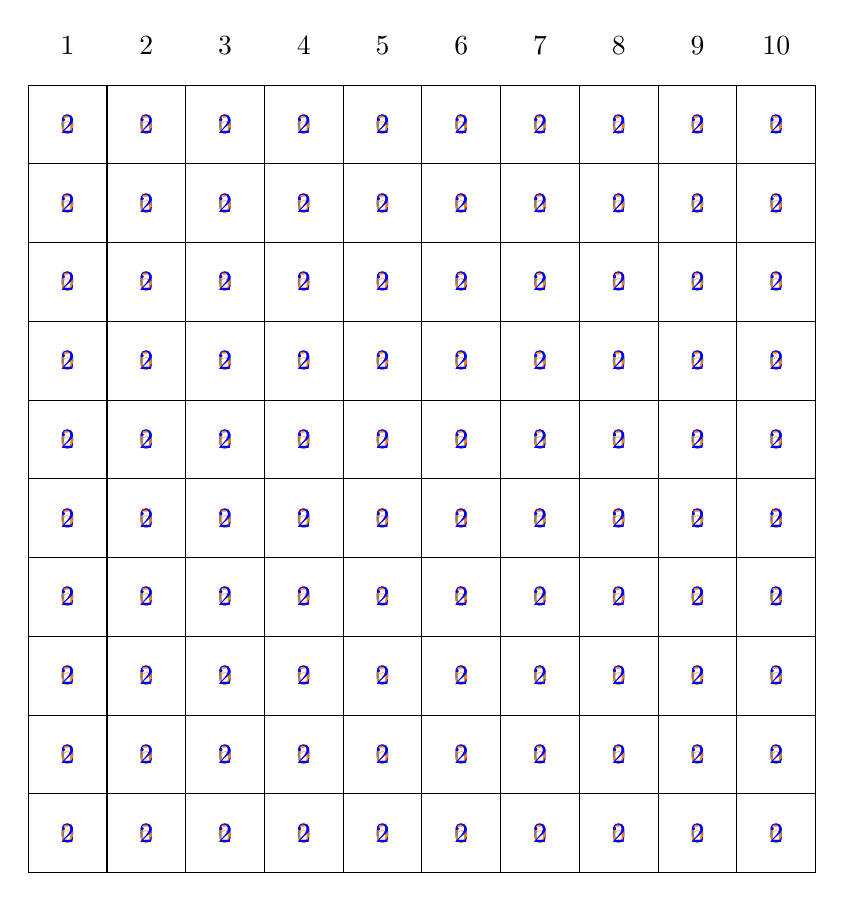
\begin{tikzpicture}
    \foreach \x in {1,...,10} {
        \draw (\x + 0.5, 11.5) node {\x};
    }
    \foreach \x in {1,...,10} {
        \foreach \y in {1,...,10} {
            \draw (\x, \y) rectangle (\x +1, \y +1);
            \ifnumcomp{\x}{<}{3}{
                \draw[color=gray] (\x +0.5, \y +0.5) node {0};
            }{
                \ifnumcomp{\y}{>}{7}{
                    \draw[color=gray] (\x +0.5, \y +0.5) node {0};
                }{
                    \ifnumcomp{\y}{<}{6}{
                        \ifnumcomp{\x}{>}{4}{
                            \draw[color=orange] (\x +0.5, \y +0.5) node {5};
                        }{
                            \draw[color=blue] (\x +0.5, \y +0.5) node {2};
                        }                                                    
                    }{
                        \draw[color=blue] (\x +0.5, \y +0.5) node {2};
                    }                      
                }
            }
        }
    }
    \end{tikzpicture}
}